\documentclass[conference]{IEEEtran}
\IEEEoverridecommandlockouts
% The preceding line is only needed to identify funding in the first footnote. If that is unneeded, please comment it out.
\usepackage{cite}
\usepackage{amsmath,amssymb,amsfonts}
\usepackage{algorithmic}
\usepackage{graphicx}
\usepackage{textcomp}
\usepackage{xcolor}
% --- Added for System Design / Prompt Composition section (diagrams, tables, code) ---
\usepackage[utf8]{inputenc}
\usepackage[T1]{fontenc}
\usepackage{booktabs}
\usepackage{listings}
\usepackage{subcaption}
\usepackage{tikz}
\usetikzlibrary{arrows.meta,positioning,fit,backgrounds,shapes.geometric,calc}
\lstdefinestyle{promptbox}{
  basicstyle=\scriptsize\ttfamily,
  breaklines=true,
  breakatwhitespace=false,
  columns=fullflexible,
  keepspaces=true,
  frame=single,
  framerule=0.3pt,
  framesep=5pt,
  xleftmargin=6pt,
  xrightmargin=3pt,
  aboveskip=6pt,
  belowskip=4pt,
}
% ------------------------------------------------------------------------------------
\def\BibTeX{{\rm B\kern-.05em{\sc i\kern-.025em b}\kern-.08em
    T\kern-.1667em\lower.7ex\hbox{E}\kern-.125emX}}
\begin{document}

\title{Towards an LLM-based Conversational Tutor for Scratch Programming in Children
}

\author{\IEEEauthorblockN{1\textsuperscript{st} Given Name Surname}
\IEEEauthorblockA{\textit{dept. name of organization (of Aff.)} \\
\textit{name of organization (of Aff.)}\\
City, Country \\
email address or ORCID}
\and
\IEEEauthorblockN{2\textsuperscript{nd} Given Name Surname}
\IEEEauthorblockA{\textit{dept. name of organization (of Aff.)} \\
\textit{name of organization (of Aff.)}\\
City, Country \\
email address or ORCID}
\and
\IEEEauthorblockN{3\textsuperscript{rd} Given Name Surname}
\IEEEauthorblockA{\textit{dept. name of organization (of Aff.)} \\
\textit{name of organization (of Aff.)}\\
City, Country \\
email address or ORCID}
\and
\IEEEauthorblockN{4\textsuperscript{th} Given Name Surname}
\IEEEauthorblockA{\textit{dept. name of organization (of Aff.)} \\
\textit{name of organization (of Aff.)}\\
City, Country \\
email address or ORCID}
\and
\IEEEauthorblockN{5\textsuperscript{th} Given Name Surname}
\IEEEauthorblockA{\textit{dept. name of organization (of Aff.)} \\
\textit{name of organization (of Aff.)}\\
City, Country \\
email address or ORCID}
\and
\IEEEauthorblockN{6\textsuperscript{th} Given Name Surname}
\IEEEauthorblockA{\textit{dept. name of organization (of Aff.)} \\
\textit{name of organization (of Aff.)}\\
City, Country \\
email address or ORCID}
}

\maketitle

\begin{abstract}
This document is a model and instructions for \LaTeX.
This and the IEEEtran.cls file define the components of your paper [title, text, heads, etc.]. *CRITICAL: Do Not Use Symbols, Special Characters, Footnotes,
or Math in Paper Title or Abstract.
\end{abstract}

\begin{IEEEkeywords}
component, formatting, style, styling, insert
\end{IEEEkeywords}

\section{Introduction}
Computational thinking (CT) has emerged as a foundational competence for the twenty-first century, encompassing problem decomposition, abstraction, pattern recognition, and algorithmic reasoning [Wing, 2006]. Introducing CT in primary education has become a global priority, and visual programming environments such as Scratch [Resnick et al., 2009] have proven effective for developing these skills in young learners, providing a low-floor entry point where children can construct programs by connecting blocks rather than writing text. Brennan and Resnick's framework [2012] identifies computational concepts, practices, and perspectives that emerge through this kind of construction, and has become a widely adopted lens for evaluating CT development in children.
Despite the accessibility of Scratch, developing CT in classroom settings remains challenging. Instructors often support many children simultaneously, and requests for help accumulate faster than they can be individually addressed. Learners who become confused or stuck often disengage before receiving guidance, and instructors report difficulty identifying which children need immediate attention. Individualized scaffolding, widely recognized as central to effective learning [Wood et al., 1976; VanLehn, 2011], is difficult to sustain under these conditions, particularly for children aged 8 to 10, whose metacognitive skills are still developing and who may not know how to ask for help productively.
Large Language Models (LLMs) present an opportunity to complement instructor attention through conversational tutoring aligned with CT learning goals. Recent work has explored LLM-based tutors for programming education [CITE 1-2], but most target adult learners, text-based languages, or assume typing fluency and metacognitive skills that primary-school children have not yet fully developed. Designing an LLM tutor to support CT development in this age group introduces distinct challenges: (i) the child's expressive capacity is limited by typing and vocabulary, requiring scaffolded interaction rather than open-ended dialogue; (ii) the tutor must recognize the child's stage in the CT construction process and respond appropriately without displacing the learner's reasoning; and (iii) the tutor must operate within tight cost constraints to be sustainable in educational programs at scale.
The introduction of LLMs in educational contexts has also raised concerns. Critics argue that reliance on AI-generated responses may reduce learners' opportunities for productive struggle Kirschner \& Hendrick, 2020, weaken metacognitive engagement, and encourage cognitive offloading in ways that erode long-term skill acquisition [Gerlich, 2025; Kosmyna et al., 2025]. In programming education specifically, studies have documented that unrestricted access to code-generating assistants can lead learners to accept solutions without understanding them, undermining core CT skills such as decomposition and debugging [CITE Prather et al.; Denny et al.]. These concerns are particularly salient for young learners, whose CT skills are still forming and whose reliance on external cognitive support may become habitual. An LLM-based tutor designed for this population must therefore be intentional about when and how it intervenes, prioritizing scaffolding over solution delivery, and preserving space for the learner's own reasoning.
In this paper we present the design and technical evaluation of a web-based conversational tutor intended to support CT development in children aged 9 to 12 as they build Scratch projects. Guided by scaffolding theory [Wood et al., 1976] and predict-observe-explain instructional strategies [White \& Gunstone, 1992], and mindful of the risks outlined above, our design articulates four explicit interaction phases (predict, hint, confirm, respond) and a progressive hint mechanism that supports learners without prematurely revealing solutions. The system is implemented with structured LLM outputs and validated block suggestions to prevent hallucination, and its token footprint is optimized for sustainable deployment.


\section{Related work}
\section{System Design}

The tutor is designed as an integrated system that combines four components: the user interface (UI), the interaction logic, the exercise representation, and the LLM prompt. These components were designed together to keep the tutor focused on the learner's current programming task while providing consistent guidance.

Four design decisions guided the implementation.
Exercise-bounded interaction. The tutor supports one programming exercise at a time instead of acting as a general-purpose programming assistant. Each exercise defines the learning objective, the relevant computational thinking concepts, and the expected solution strategy. Limiting the interaction to this context keeps the tutor focused on the learner's current task, reduces off-topic conversation, and makes the generated feedback easier to evaluate against well-defined learning objectives.

Structured and validated output. The tutor never returns free-form text alone. Each turn yields a typed object that carries a pedagogical phase, a short message for the child, an optional set of Scratch blocks to show, and two or three reply options. The model receives the full catalog of available blocks and may name only blocks that appear in it; the backend then removes any block the model invents before the reply reaches the child. This keeps every suggestion faithful to the Scratch environment and prevents the tutor from pointing to instructions that do not exist.

Phase-based scaffolding with progressive hints. The interaction is organized around four phases that follow how a human tutor moves a learner forward: predict, hint, confirm, and respond. When a child asks for help, the tutor first invites a prediction about what a block does; if the child stays stuck, it releases progressively more concrete hints, from a nudge toward a category of blocks to a description of the block to be used, and only as a last step to the block itself. A reference solution guides this escalation but is withheld from the child, so the learner keeps ownership of the reasoning rather than receiving the answer.

Latency- and cost-aware operation. Young learners disengage when a reply takes too long, so the system favors a fast model with a compact prompt over a larger and slower one. Each request carries only the last fourteen messages of the conversation, a trimmed block catalog, and a low sampling temperature. We deploy Gemini~2.5~Flash rather than a heavier reasoning-oriented model because the extra deliberation time of the latter pushed response latency past what a child of this age will wait through, without a matching gain in tutoring quality for these short exchanges. The backend also records input and output token counts per message, which makes the running cost measurable and keeps the design accountable to the sustainability constraint stated in the introduction.

\subsection{Architecture}

Fig.~\ref{fig:arch} shows the runtime architecture. The front end is a single-page React application built with Vite. Rather than a route-based structure, it runs a small five-screen state machine (welcome, assent, game selection, chat, and feedback) with the active conversation and session held in memory, and it reaches the back end through a single typed API client. This keeps the child's path through the app linear and predictable, which matters for an eight-to-ten-year-old audience.

The back end is a FastAPI service organized in four layers with a single responsibility each: routes expose the HTTP surface under \texttt{/api/v1}, services hold the tutoring logic, repositories own all database access, and models define the schema through an asynchronous SQLAlchemy mapping. The tutoring logic depends on a provider-agnostic \texttt{TutorLLM} interface, and a factory selects the concrete provider at runtime from a single configuration flag. Sessions, conversations, messages, and anonymous feedback persist to PostgreSQL in production and to SQLite during development, without any change to application code. In a deployed installation, nginx serves the compiled front end and proxies \texttt{/api/} to the back end, so the browser talks to one origin.

Fig.~\ref{fig:sequence} traces a single turn. The child either taps a reply option or types a message; the front end posts it to the conversation endpoint; the service persists the child message, assembles the prompt described in Section~\ref{sec:prompt}, and calls the selected model; the reply is validated against the block catalog, stored with its phase and token counts, and returned to the front end, which renders the message together with its phase cue, any block cards, and the next set of reply options.

\begin{figure*}[!t]
\centering
\resizebox{\textwidth}{!}{%
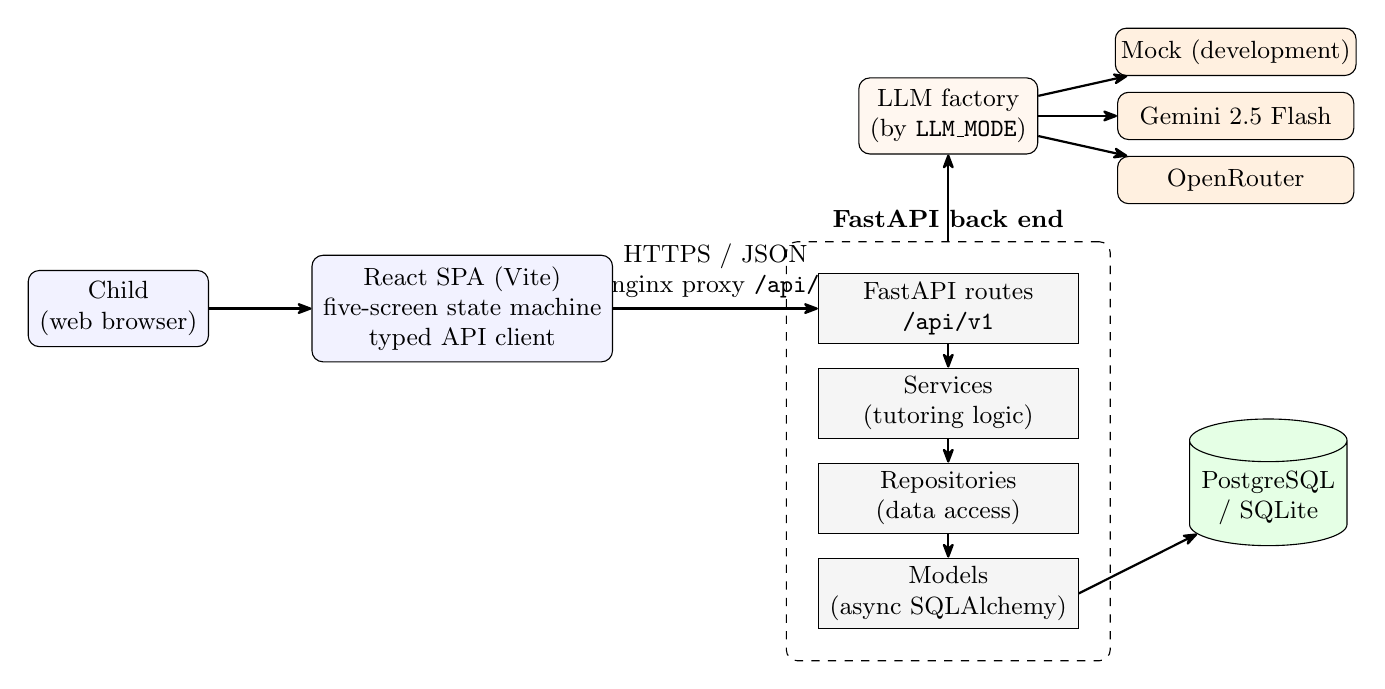
\begin{tikzpicture}[
  font=\small,
  >={Stealth[round]},
  box/.style={draw, rounded corners, align=center, minimum height=9mm, inner sep=4pt, fill=blue!5},
  layer/.style={draw, align=center, minimum width=33mm, minimum height=7mm, fill=gray!8, inner sep=3pt},
  db/.style={draw, cylinder, shape border rotate=90, aspect=0.28, align=center, minimum height=13mm, minimum width=20mm, fill=green!10},
  prov/.style={draw, rounded corners, align=center, minimum width=30mm, minimum height=6mm, fill=orange!12, inner sep=2pt},
  arr/.style={-{Stealth[round]}, thick},
]
% client side
\node[box] (child) {Child\\(web browser)};
\node[box, right=13mm of child] (spa) {React SPA (Vite)\\five-screen state machine\\typed API client};
% backend internal layers
\node[layer, right=26mm of spa] (routes) {FastAPI routes\\\texttt{/api/v1}};
\node[layer, below=3mm of routes] (svc) {Services\\(tutoring logic)};
\node[layer, below=3mm of svc] (repo) {Repositories\\(data access)};
\node[layer, below=3mm of repo] (model) {Models\\(async SQLAlchemy)};
\begin{scope}[on background layer]
\node[draw, dashed, rounded corners, fit=(routes)(svc)(repo)(model), inner sep=4mm] (be) {};
\end{scope}
\node[above=0.5mm of be.north] {\textbf{FastAPI back end}};
% persistence
\node[db, right=14mm of repo] (dbn) {PostgreSQL\\/ SQLite};
% llm providers
\node[box, above=11mm of be.north, fill=orange!6] (factory) {LLM factory\\(by \texttt{LLM\_MODE})};
\node[prov, right=10mm of factory] (gem) {Gemini 2.5 Flash};
\node[prov, above=2mm of gem] (mock) {Mock (development)};
\node[prov, below=2mm of gem] (orr) {OpenRouter};
% arrows
\draw[arr] (child) -- (spa);
\draw[arr] (spa) -- node[above, align=center]{HTTPS / JSON\\nginx proxy \texttt{/api/}} (routes.west);
\draw[arr] (routes) -- (svc);
\draw[arr] (svc) -- (repo);
\draw[arr] (repo) -- (model);
\draw[arr] (model.east) -- (dbn);
\draw[arr] (be.north) -- (factory.south);
\draw[arr] (factory) -- (gem);
\draw[arr] (factory) -- (mock);
\draw[arr] (factory) -- (orr);
\end{tikzpicture}%
}
\caption{Runtime architecture. A React single-page application drives a linear five-screen flow and communicates with a layered FastAPI back end over JSON. The tutoring logic calls a provider-agnostic language-model interface whose concrete implementation is selected by a single configuration flag; sessions and messages persist to PostgreSQL in production and SQLite in development.}
\label{fig:arch}
\end{figure*}

\begin{figure}[!t]
\centering
\resizebox{\columnwidth}{!}{%
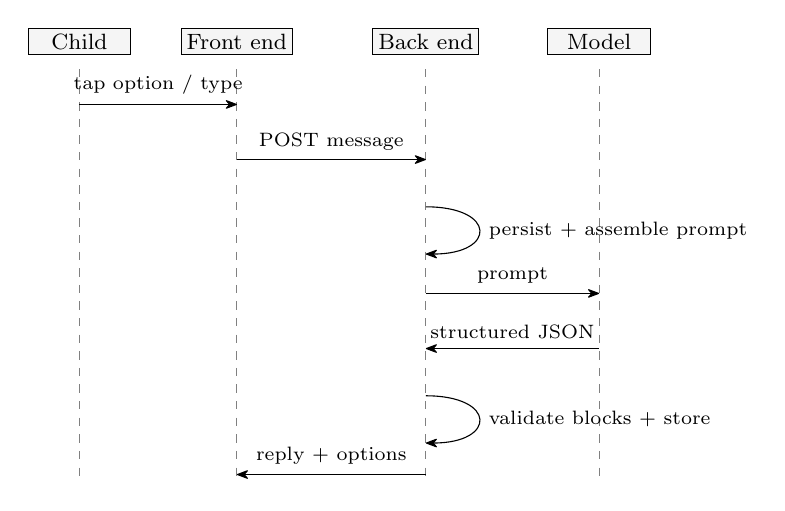
\begin{tikzpicture}[font=\footnotesize, >={Stealth[round]}]
% lifelines
\foreach \x/\name in {0/Child, 2.0/Front end, 4.4/Back end, 6.6/Model}{
  \node[draw, fill=gray!8, minimum width=13mm, inner sep=2pt] (h\name) at (\x,0) {\name};
  \draw[dashed, gray] (\x,-0.35) -- (\x,-5.6);
}
\draw[-{Stealth[round]}] (0,-0.8) -- node[above, font=\scriptsize]{tap option / type} (2.0,-0.8);
\draw[-{Stealth[round]}] (2.0,-1.5) -- node[above, font=\scriptsize]{POST message} (4.4,-1.5);
% backend self action
\draw[-{Stealth[round]}] (4.4,-2.1) .. controls (5.3,-2.1) and (5.3,-2.7) .. (4.4,-2.7)
  node[right, font=\scriptsize, pos=0.5]{persist + assemble prompt};
\draw[-{Stealth[round]}] (4.4,-3.2) -- node[above, font=\scriptsize]{prompt} (6.6,-3.2);
\draw[{Stealth[round]}-] (4.4,-3.9) -- node[above, font=\scriptsize]{structured JSON} (6.6,-3.9);
\draw[-{Stealth[round]}] (4.4,-4.5) .. controls (5.3,-4.5) and (5.3,-5.1) .. (4.4,-5.1)
  node[right, font=\scriptsize, pos=0.5]{validate blocks + store};
\draw[{Stealth[round]}-] (2.0,-5.5) -- node[above, font=\scriptsize]{reply + options} (4.4,-5.5);
\end{tikzpicture}%
}
\caption{Message exchange for one turn. The back end persists the child message, assembles the layered prompt, calls the model, and validates the block suggestions against the catalog before storing and returning the typed reply.}
\label{fig:sequence}
\end{figure}

\subsection{Language Models}
\label{sec:models}

The default provider is Google Gemini~2.5~Flash. It is called with a native structured-output schema, so the model is constrained to emit the typed reply object directly rather than free text that the back end would have to parse. Sampling temperature is held at 0.3 to keep tutoring behavior stable across turns. A second provider routes the same prompt through the OpenRouter API using an OpenAI-compatible interface; because that path does not expose a native schema, the prompt appends an explicit description of the required JSON object. A mock provider returns deterministic replies with no network call and is used for local development and automated tests. All three implement the same \texttt{TutorLLM} interface and are interchangeable through configuration, which let us compare providers without touching the tutoring logic.

\section{Prompt Composition}
\label{sec:prompt}

The behavior of the tutor is defined almost entirely by how the prompt is assembled. Each request combines a fixed pedagogical instruction, a description of the current exercise, the catalog of usable blocks, and the recent conversation, and it constrains the model to answer with a typed object. Table~\ref{tab:prompt} lists these parts, and Fig.~\ref{fig:prompt} shows how they are layered into one request and how the reply flows back to the interface.

\begin{table}[!t]
\caption{Components of the assembled prompt}
\label{tab:prompt}
\centering
\renewcommand{\arraystretch}{1.25}
\begin{tabular}{@{}p{1.7cm}p{1.4cm}p{3.7cm}@{}}
\toprule
\textbf{Component} & \textbf{Scope} & \textbf{Purpose} \\
\midrule
Static base & Every turn & Persona, four-phase policy, progressive-hint rule, block and reply-option rules \\
Exercise context & Per exercise & Title, child instruction, objectives, hints; and, privately, the reference solution and key-block ids \\
Block catalog & Every turn & The 47 available blocks (id, name, description) as the only allowed vocabulary \\
Transcript & Every turn & The last 14 messages plus the new child message \\
Output schema & Every turn & Six typed fields the model must return \\
\bottomrule
\end{tabular}
\end{table}

\begin{figure*}[!t]
\centering
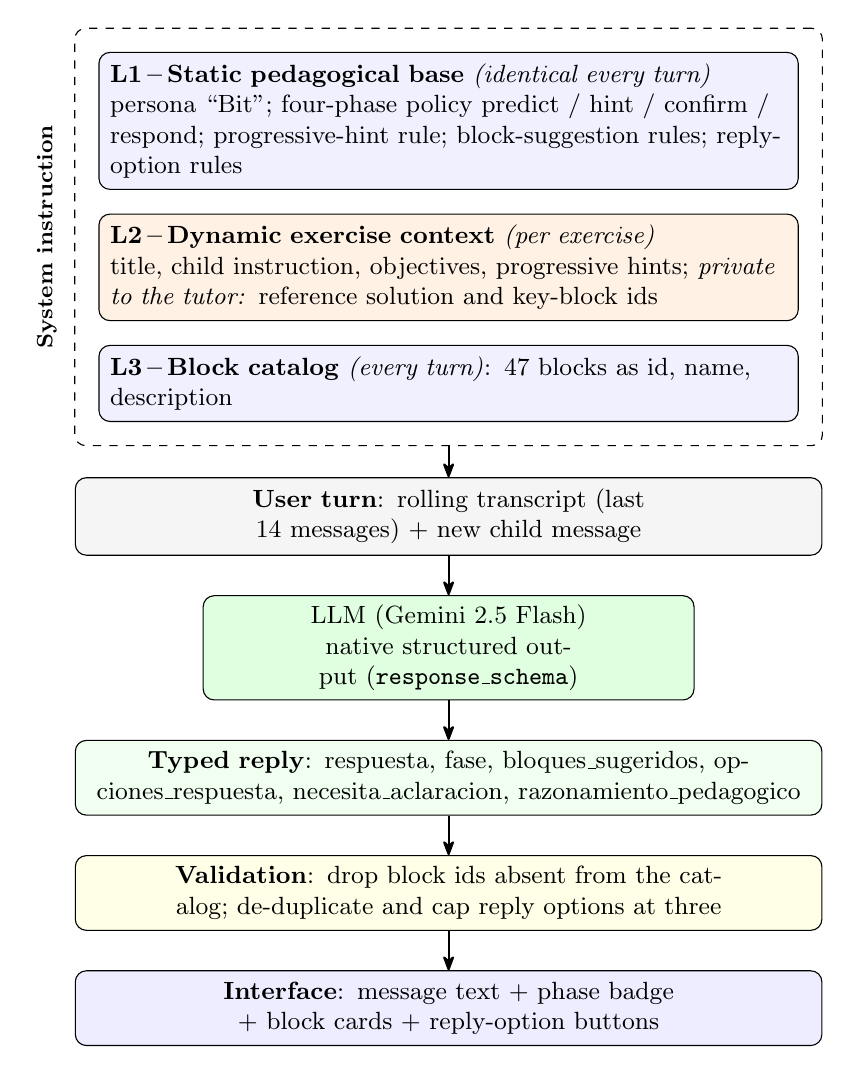
\begin{tikzpicture}[
  font=\small,
  >={Stealth[round]},
  node distance=3mm,
  layerA/.style={draw, rounded corners, align=left, text width=86mm, fill=blue!6, inner sep=4pt},
  layerB/.style={draw, rounded corners, align=left, text width=86mm, fill=orange!10, inner sep=4pt},
  io/.style={draw, rounded corners, align=center, text width=92mm, fill=gray!8, inner sep=4pt},
  llm/.style={draw, rounded corners, align=center, text width=60mm, fill=green!12, minimum height=9mm},
  arr/.style={-{Stealth[round]}, thick},
]
\node[layerA] (base) {\textbf{L1\,--\,Static pedagogical base} \emph{(identical every turn)}\\ persona ``Bit''; four-phase policy predict / hint / confirm / respond; progressive-hint rule; block-suggestion rules; reply-option rules};
\node[layerB, below=of base] (ctx) {\textbf{L2\,--\,Dynamic exercise context} \emph{(per exercise)}\\ title, child instruction, objectives, progressive hints; \emph{private to the tutor:} reference solution and key-block ids};
\node[layerA, below=of ctx] (cat) {\textbf{L3\,--\,Block catalog} \emph{(every turn)}: 47 blocks as id, name, description};
\begin{scope}[on background layer]
\node[draw, dashed, rounded corners, fit=(base)(ctx)(cat), inner sep=3mm] (sys) {};
\end{scope}
\node[left=1mm of sys.west, rotate=90, anchor=south, font=\footnotesize\bfseries] {System instruction};
\node[io, below=7mm of cat] (turn) {\textbf{User turn}: rolling transcript (last 14 messages) $+$ new child message};
\node[llm, below=5mm of turn] (llm) {LLM (Gemini 2.5 Flash)\\ native structured output (\texttt{response\_schema})};
\node[io, below=5mm of llm, fill=green!6] (json) {\textbf{Typed reply}: respuesta, fase, bloques\_sugeridos, opciones\_respuesta, necesita\_aclaracion, razonamiento\_pedagogico};
\node[io, below=5mm of json, fill=yellow!10] (val) {\textbf{Validation}: drop block ids absent from the catalog; de-duplicate and cap reply options at three};
\node[io, below=5mm of val, fill=blue!7] (ui) {\textbf{Interface}: message text $+$ phase badge $+$ block cards $+$ reply-option buttons};
\draw[arr] (sys.south) -- (turn.north);
\draw[arr] (turn) -- (llm);
\draw[arr] (llm) -- (json);
\draw[arr] (json) -- (val);
\draw[arr] (val) -- (ui);
\end{tikzpicture}
\caption{Prompt composition and reply flow. The system instruction is assembled from a static pedagogical base, the current exercise context (whose reference solution and key blocks stay hidden from the child), and the block catalog. Together with the recent transcript it forms one request; the model returns a typed object that the back end validates against the catalog before the interface renders it.}
\label{fig:prompt}
\end{figure*}

\subsection{Static Pedagogical Base}

The static base is the same on every turn and encodes the tutor's persona and its rules of engagement. It casts the model as ``Bit,'' a friendly Scratch tutor for children, and states the governing goal plainly: help the learner understand, do not solve the exercise for them. It then maps common situations to the four phases, for example a greeting or a factual question maps to \emph{respond}, a first request for help maps to \emph{predict}, and repeated difficulty maps to escalating \emph{hint}. The base also fixes surface constraints that matter for this audience: short sentences, at most one emoji, no more than one block shown per turn, and an explicit reminder that the tutor cannot see the child's screen and must ask when it needs to know what the child has built.

\subsection{Dynamic Exercise Context}

For each exercise the back end appends a compact context block. It always includes the title, the child-facing instruction, the learning objectives, and the author-written progressive hints. When the exercise defines them, it also adds two fields that are marked as private and are never to be revealed in full: a natural-language reference solution and an ordered list of key block ids. The reference solution acts as a compass for deciding the next step and the next question to ask, and the key blocks tell the tutor which ids to prefer when a suggestion is warranted. Listing~\ref{lst:ctx} shows this context for a representative exercise, translated from the Spanish used in deployment.

\begin{lstlisting}[style=promptbox, caption={Exercise context for a representative game (translated; block ids are verbatim).}, label={lst:ctx}]
CURRENT EXERCISE:
Title: Make the cat dance
Child instruction: Let's make the cat dance!
  First think: which block makes the program start?
Objectives: use the green-flag event; move and
  turn the sprite; use repetition to animate.
Progressive hints:
  1) Look in the Events category to start.
  2) In Motion there are blocks that turn and move.
  3) To really dance, use Repeat from Control.

REFERENCE SOLUTION (for you only, do not reveal
  it in full; use it as a compass): on green flag,
  the cat moves right then left several times in a
  loop with short waits, then spins and faces right.

KEY BLOCKS (for you only, prefer these ids, show
  one per turn):
  - eventos_bandera_verde ("green flag")
  - movimiento_mover_pasos ("move steps")
  - movimiento_girar_derecha_grados ("turn right")
  - control_repetir_veces ("repeat times")
  - control_por_siempre ("forever")
\end{lstlisting}

\subsection{Block Catalog and Anti-Hallucination Grounding}

Every request carries a trimmed catalog of the 47 Scratch blocks the tutor may reference, each with an id, a display name, and a one-line description. The catalog serves two purposes. It gives the model a closed vocabulary so that suggestions stay inside the blocks a child actually has, and it anchors the ids that the back end later checks. After the model answers, the back end keeps only the suggested blocks whose ids appear in the catalog and discards the rest, so an invented or misspelled block never reaches the interface. The same id is used to look up the block image the child sees, which ties the textual suggestion to a concrete visual element in Scratch.

\subsection{Structured Output Contract}

The prompt requires the model to answer with a single typed object rather than prose. Its fields are the message shown to the child (\texttt{respuesta}), the pedagogical phase (\texttt{fase}), the blocks to display (\texttt{bloques\_sugeridos}), the reply options (\texttt{opciones\_respuesta}), a flag indicating the tutor needs to see more before it can help (\texttt{necesita\_aclaracion}), and a short internal note explaining the pedagogical choice (\texttt{razonamiento\_pedagogico}) that is logged but not shown. Listing~\ref{lst:json} gives the schema. Because the phase is part of the output, the tutor declares on every turn where it stands in the scaffolding cycle, which the interface renders as a colored badge and which also makes each turn analyzable after the fact. Fig.~\ref{fig:phases} shows the transitions among phases.

\begin{lstlisting}[style=promptbox, caption={Typed reply the model must return.}, label={lst:json}]
{
  "respuesta": "text shown to the child",
  "fase": "predecir" | "pista" | "confirmar" | "responder",
  "bloques_sugeridos": [{"id": "...", "imagen": "...", "nombre": "..."}],
  "opciones_respuesta": ["...", "..."],
  "necesita_aclaracion": true | false,
  "razonamiento_pedagogico": "brief internal note (not shown)"
}
\end{lstlisting}

\begin{figure}[!t]
\centering
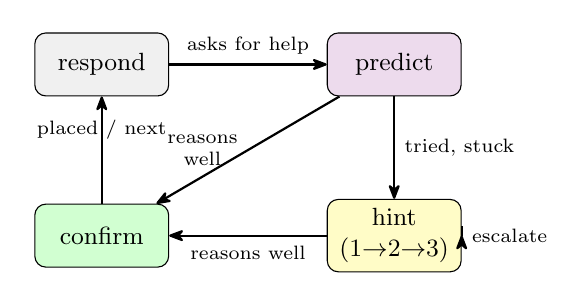
\begin{tikzpicture}[
  font=\small,
  >={Stealth[round]},
  st/.style={draw, rounded corners, align=center, minimum width=17mm, minimum height=8mm},
  arr/.style={-{Stealth[round]}, thick},
]
\node[st, fill=gray!12] (respond) {respond};
\node[st, fill=violet!14, right=20mm of respond] (predict) {predict};
\node[st, fill=yellow!22, below=13mm of predict] (hint) {hint\\(1$\to$2$\to$3)};
\node[st, fill=green!18, left=20mm of hint] (confirm) {confirm};
\draw[arr] (respond) -- node[above, font=\scriptsize]{asks for help} (predict);
\draw[arr] (predict) -- node[right, font=\scriptsize]{tried, stuck} (hint);
\draw[arr] (hint.east) to[out=-35,in=35,looseness=6] node[right, font=\scriptsize]{escalate} (hint.east);
\draw[arr] (hint) -- node[below, font=\scriptsize]{reasons well} (confirm);
\draw[arr] (predict) -- node[left, font=\scriptsize, align=center]{reasons\\well} (confirm);
\draw[arr] (confirm) -- node[above, font=\scriptsize]{placed / next} (respond);
\end{tikzpicture}
\caption{Interaction phases. A request for help moves the tutor from \emph{respond} into \emph{predict}; sustained difficulty escalates hints from vague to concrete; once the child reasons correctly the tutor \emph{confirms} and shows the block, then returns to \emph{respond}. Casual or factual turns stay in \emph{respond}.}
\label{fig:phases}
\end{figure}

\subsection{Provider-Specific Rendering}

The pedagogical base, exercise context, block catalog, and transcript are shared across providers, which keeps tutor behavior consistent when the model changes. The two providers differ only in how the output contract is enforced. Gemini is given the schema as a native response format, so the constraint is applied by the model runtime. OpenRouter, reached through an OpenAI-compatible interface, receives the same schema as an explicit instruction appended to the base and is asked to return only that object. In both cases the back end parses the result, applies the block and option validation described above, and records the provider, model, prompt version, and token counts alongside the stored message.

\section{Interaction Features}
\label{sec:features}

Four features carry the scaffolding design into the interface. Fig.~\ref{fig:ui} illustrates them in the running system.

\emph{Progressive hints.} When a child stays stuck, the tutor does not repeat itself or reveal the answer. It escalates along three levels, from a nudge toward a category of blocks, to a description of the block to look for, to showing the block itself, and only the last level places a block in the reply. The reference solution steers the escalation while remaining hidden, so support increases without removing the child's work.

\emph{Response options as scaffolding.} Under each tutor message the interface shows two or three short buttons phrased in the child's own voice, for example ``The cat moves'' or ``Give me another hint.'' The buttons lower the cost of replying for a learner who cannot yet type fluently, and one option is always an escape for the child who does not know, such as ``I'm not sure.'' A free-text field remains available for children who prefer to write their own answer, so the options guide without constraining.

\emph{Predict and verify.} Before a block is trusted, the tutor invites the child to predict what it will do and then to test it by running the program. This turns each suggested block into a small experiment rather than an instruction to copy, which keeps the child observing and reasoning about behavior in Scratch.

\emph{Validated block suggestions.} A suggested block appears as a visual card with the block image and its name, drawn from the same catalog the model is constrained to. Because the back end has already discarded any id outside the catalog, the child only ever sees blocks that exist in their environment, and the phase badge above the message signals whether the tutor is asking for a prediction, giving a hint, or confirming a step.

The surrounding flow supports classroom use. A session resumes automatically if the child closes the browser before finishing, so an interruption does not lose progress; a session is marked complete only when a teacher enters an administrator code, which keeps completion under the instructor's control; and each exercise offers an optional short video that previews the finished project.

\begin{figure*}[!t]
\centering
% --- Interaction screenshots: replace the placeholders below with captures from the running app. ---
% Expected files (place them next to this .tex, e.g. in ./fig/):
%   fig/ui_predict.png      fig/ui_hint_block.png      fig/ui_options.png      fig/ui_confirm.png
\begin{subfigure}[t]{0.48\textwidth}
  \centering
  \fbox{\rule{0pt}{42mm}\rule{0.9\linewidth}{0pt}} % placeholder box; delete when adding the image
  % \includegraphics[width=0.95\linewidth]{fig/ui_predict.png}
  \caption{Predict phase: the tutor shows one block and asks the child to predict what it does; reply options appear below.}
  \label{fig:ui-predict}
\end{subfigure}
\hfill
\begin{subfigure}[t]{0.48\textwidth}
  \centering
  \fbox{\rule{0pt}{42mm}\rule{0.9\linewidth}{0pt}} % placeholder box; delete when adding the image
  % \includegraphics[width=0.95\linewidth]{fig/ui_hint_block.png}
  \caption{Hint phase (level 3): after sustained difficulty, the tutor shows the concrete block as a validated card.}
  \label{fig:ui-hint}
\end{subfigure}

\vspace{3mm}

\begin{subfigure}[t]{0.48\textwidth}
  \centering
  \fbox{\rule{0pt}{42mm}\rule{0.9\linewidth}{0pt}} % placeholder box; delete when adding the image
  % \includegraphics[width=0.95\linewidth]{fig/ui_options.png}
  \caption{Response options as scaffolding: child-voiced buttons, including an escape option, with a free-text field kept available.}
  \label{fig:ui-options}
\end{subfigure}
\hfill
\begin{subfigure}[t]{0.48\textwidth}
  \centering
  \fbox{\rule{0pt}{42mm}\rule{0.9\linewidth}{0pt}} % placeholder box; delete when adding the image
  % \includegraphics[width=0.95\linewidth]{fig/ui_confirm.png}
  \caption{Confirm phase: once the child reasons correctly, the tutor confirms and shows the matching block.}
  \label{fig:ui-confirm}
\end{subfigure}
\caption{The tutor interface during a session (see Section~\ref{sec:features}). Each panel shows a phase badge, the tutor message, any validated block cards, and the reply options the child can tap.}
\label{fig:ui}
\end{figure*}


\end{document}
